%% V1.0
%% by Gabriel Garcia, gabrcg@gmail.com
%% This is a template for Udacity projects using IEEEtran.cls

%% Be Udacious!

\documentclass[10pt,journal,compsoc]{IEEEtran}

\usepackage[pdftex]{graphicx}    
\usepackage{cite}
\usepackage{hyperref}
\usepackage{subcaption}
% \hyphenation{op-tical net-works semi-conduc-tor}

\begin{document}

\title{Map My World}

\author{Lucas Wohlhart}

\markboth{Localization project, Robotics Nanodegree Program, Udacity}%
{}
\IEEEtitleabstractindextext{%

\begin{abstract}
In this project techniques to solve the  crucial task of simultaneous localization and mapping (SLAM) will be explored. For this purpose a robot, previously designed for a localization project\cite{LWMSE6botLocalization}, is extended with regards to it's sensory capabilities. Additionally to its laser based range scanner, IMU and wheel encoders an RGB-D camera is mounted. The SLAM method used is based on RTAB-Map Real-Time Appearance-Based Mapping proposed in \cite{LabbeRTABMap}, which is graph SLAM algorithm implementing vision-based loop closure detection. To evaluate its performance, the aforementioned robot is placed in two different simulated environments, one of which is provided by Udacity and the other is created within this project. The robot is then teleoperated through the world and creates a 2D occupancy grid map and a 3D map using the SLAM algorithm.

\end{abstract}

% Note that keywords are not normally used for peerreview papers.
\begin{IEEEkeywords}
Robot, IEEEtran, Udacity, \LaTeX, Localization.
\end{IEEEkeywords}}


\maketitle
\IEEEdisplaynontitleabstractindextext
\IEEEpeerreviewmaketitle
\section{Introduction}
\label{sec:introduction}
% Introduction - Explain the concept of the project and what is trying to be achieved.
% Introduction - Student can clearly and accurately explain the problem domain.

\IEEEPARstart{T}{he} task of simultaneous localization and mapping (SLAM) is of utmost importance for the field of robotics. In the vast majority of realworld applications one cannot provide a predetermined map of the environment a robot is acting in, which is a necessity for localization and path planning. Apart from the initial nonexistence of a map, a robot also frequently operates in dynamic sceneries which means that existing maps have to be altered to accommodate changes. Therefore a map has to be generated on the fly using adequate sensors. Since the robots location is generally also unknown, SLAM can certainly be considered a chicken or egg problem.

There are various approaches to solving the SLAM problem such as Occupancy grid mapping, Fast-SLAM and GraphSLAM. The method studied in detail in this project is RTAB-Mapping (Real-Time Appearance-Based Mapping) which is a graph-based method utilizing a rangefinder sensor and an RGB-D camera.

The goal of the project is the creation of satisfactory mappings of two simulated environments by teleoperating a robot through them and estimating a 2D occupancy grid and a 3D map of the world using its sensors and the RTAB-Map algorithm.


\section{Background}

As previously described the SLAM problem is a very important aspect of mobile robotics especially for localization, planning and obstacle avoidance. Therefore the research community has come up with a plethora of methods to tackle this challenging task.

SLAM itself is divided into two different problem sets. Solving the so called online SLAM problem means estimating the current pose and map based only on current measurements and controls, whereas full SLAM poses the challenge of estimating the entire trajectory of poses a robot has passed through and a map based all previous and current measurements and controls.
Since the estimated map is based on the estimated poses and vice versa, these estimates have to be optimized jointly. Facing a vast hypothesis space, unavoidable sensor noise and perceptual ambiguity of detectable features makes solving the SLAM problem hard.

The following list gives a quick overview over some of the methods used to solve this challenging task.

\subsection{Occupancy Grid Map}

The occupancy grid mapping algorithm divides the mappable space into a grid of evenly spaced cells. Each grid cell represents an independent binary random variable indicating the probability of the location being occupied or free. When a robot moves through an environment and senses its surroundings, the sensor data is projected to the grid map domain where it is used to update the occupancy probability of the observed cells. The readings of a range sensor, such as a laser- or a sonic range finder can for example provide evidence that the cells up to the point of reflection are free and that there's an obstacle at the reflection point. This kind of sensor data is usually modelled with a cone, depicted in Fig.\ref{fig:occupancy_grid_sensor_model}, to account for sensor specific uncertainties.
The occupancy grid map algorithm uses log-odds to model the cell probabilities,providing numerical stability and allowing for simple addition of log-odds when performing an update on a cell. Each incoming sensor reading is used to update the cells that are currently in the field of view of the robot, leaving the others unchanged.

Since the algorithm itself doesn't provide a method to estimate the robots pose, one has to use odometry data from sensors such as the IMU, wheel encoders and/or GPS to estimate it.

\begin{figure}[thpb]
      \centering
      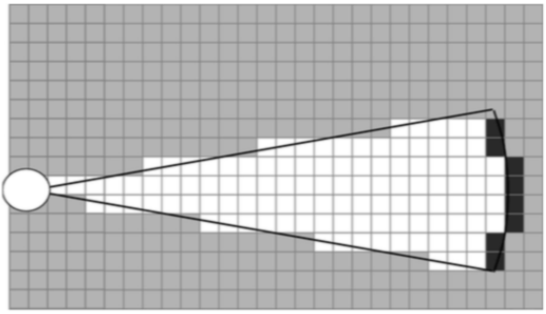
\includegraphics[width=0.4\linewidth]{img/occupancy_grid_sensor_model.png}
      \caption{Range finder sensor model (cone)}
      \label{fig:occupancy_grid_sensor_model}
\end{figure}

\subsection{FastSLAM}

The FastSLAM algorithm is based on a particle filter approach and requires known landmarks. Each particle holds a possible trajectory of the robot poses and a corresponding estimated map. The features of the map are modelled as local gaussians. 
It estimates a posterior over the robot path using a low dimensional Extended Kalman Filter to solve the independent map features. Being able to jointly estimate the robot trajectory and the map means that FastSLAM is able to solve the full SLAM problem. Every particle filter update step begins by sampling from the probabilistic motion model based on the current particles and the executed motion command yielding a temporary set of particles \cite{montemerlo_fastslam}. This particle distribution is referred to as the \textit{proposal distribution}. They model the instantaneous pose of the robot, which is why the algorithm is also capable of solving the online SLAM problem. The filter update is then completed by resampling from this newly weighted temporary particle set to achieve a joint optimization of the entire trajectory and the map.

\subsubsection{FastSLAM 1.0 and FastSLAM 2.0}
FastSLAM 1.0 is considered a powerfull tool to solve the SLAM problem, yet it is known to be sample inefficient. FastSLAM 2.0\cite{montemerlo_fastslam_2_0} improves this deficit by modifying the way the previously described proposal distribution is acquired. While the previous version of the algorithm just uses the motion commands (which is unfortunately known to be a rather noisy source of data) to sample the instantaneous pose, FastSLAM 2.0 also incorporates the current measurements to yield a more meaningfull set of particles for the following resampling step.

\subsubsection{Grid-based FastSLAM}
The Grid-based FastSLAM algorithm eliminates the necessity of predefining landmarks by combining the concept of FastSLAM with an occupancy grid approach as replacement. Each particle now holds its own grid map and each one of them is updated according to occupancy grid mapping algorithm. This enables the Grid-based FastSLAM algorithm to be applied in entirely unknown scenarios.

\subsection{Graph-SLAM}
The Graph-SLAM\cite{thrun_graph_2006} algorithm takes the different approach of constructing a graph with nodes for each motion step performed by the robot. Each node introduces a motion constraint which models the presumed motion performed to go from the previous node to the current one. Additionally it holds several measurement constraints representing the evidence gathered from sensory data, such as distances to identified landmarks. A simple example of such a graph is depicted in Fig.~\ref{fig:graph_slam_example_graph}

\begin{figure}[thpb]
    \centering
    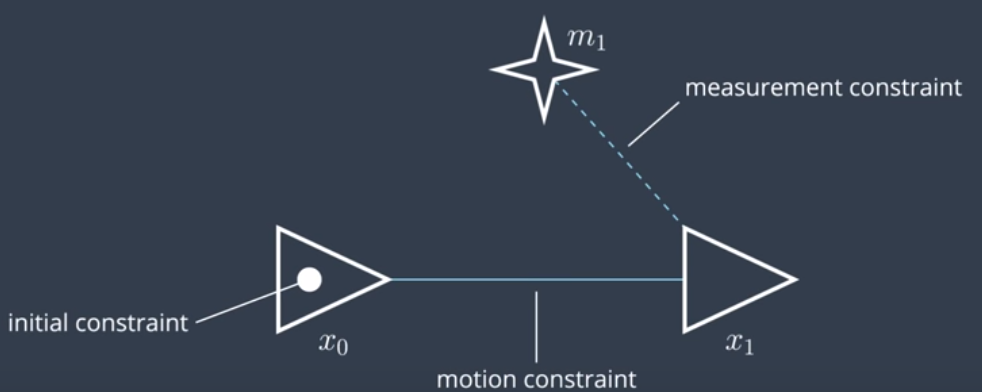
\includegraphics[width=0.9\linewidth]{img/graph_slam_example_graph.png}
    \caption{Graph-SLAM example graph \\(credits: udacity robotics nanodegree lesson 18)}
    \label{fig:graph_slam_example_graph}
\end{figure}

The so called \textit{Front-End} of the algorithm is concerned with the creation and insertion of such nodes based on motion commands, odometry data and sensor readings.
The \textit{Back-End} of GraphSLAM uses the entire graph to perform graph optimization based on maximum likelihood estimation (MLE). It tries to find the best configuration of nodes that yields the smallest error based on all the constraints introduced by all nodes. This method makes a GraphSLAM capable of solving the full SLAM problem, in a relatively efficient manner.

\subsubsection{RTAB-Map}
RTAB-Map is an RGB-D GraphSLAM method implementing Real-Time Appearance-Based Mapping with incremental vision-based loop closure detection. In appearance based methods, a robot uses visual features to localize itself which also enables the identification of previously observed locations based on matching them to stored reference features. Reencountering such known locations allows for loop closure detection which can greatly improve pose estimation and yield a more robust and coherent mapping result.

Features are usually extracted using the SURF\cite{leonardis_surf:_2006} descriptors which allows the algorithm to continously build a \textit{visual bag-of-words} by clustering the instances of these features. Newly extracted features are then compared to the existing clusters to find matches and determine the likelihood of having encountered a loop closure.

RTAB-Map is optimized for longterm, large scale SLAM and therefore implements a sophisticated memory management strategy to allow loop closure detection and graph optimization in realtime.
\begin{itemize}
    \item Short-Term Memory (STM)
    \item Working Memory (WM)
    \item Long-Term Memory (LTM)
\end{itemize}
The STM holds the most recent nodes encountered by the robot. It is not considered for loop closure detection because these nodes by nature very similar to each other. Once the amount of nodes in the Short-Term Memory exceeds is fixed size nodes are transferred to the WM.

The nodes in WM are used for loop closure detection as well as graph optimization. The amount of nodes in the WM is determined by the time it takes to perform optimization and loop closure detection. Once the realtime threshold is exceeded, nodes get transferred to LTM.

The LTM holds nodes that are not considered for loop closure detection or graph optimization, however if a loop closure is encountered, the WM can retrieve neighbouring nodes from the LTM to reactivate them for optimization.

% Background - Explain the importance of both mapping two and three dimensional space.
% Background - The student provides a sufficient background into the scope of the problem / technologically while also identifying some of the current challenges in robot mapping and why the problem domain is an important piece of robotics. They further discuss and compare mapping algorithms

\section{Scene and robot configuration}
\subsection{Scene configuration}
The personal Gazebo world, called \textit{factory\_room} was created by launching an empty world in the Gazebo simulation environment, using the building editor to construct the wall structure of the room and arranging objects provided by the Gazebo model database. The resulting environment represents a small factory or workshop with several tables, shelves, storage boxes and utilities usually encountered in such a scenario. A person is standing close to one of the desks and the outside features trees to provide visual features visible through the windows. The scene is depicted in Fig.~\ref{fig:factory_world}

Initially the walls of the room had a brickwall pattern which had to be removed due to erroneous loop detection which will be discussed in more detail in the following sections.
% Scene and robot configuration - Explain how your personal Gazebo world was created and what is the layout of it. Justify your choice of robot parameters, sensor location, and how you decided to configure your package structure.
% Scene and robot configuration - Student explains how the gazebo world was created by providing an overview of the layout of items in his/her customized Gazebo world. Student also describes the robot's parameters, sensor features, and reasoning on the package structure.

\begin{figure}[thpb]
      \centering
      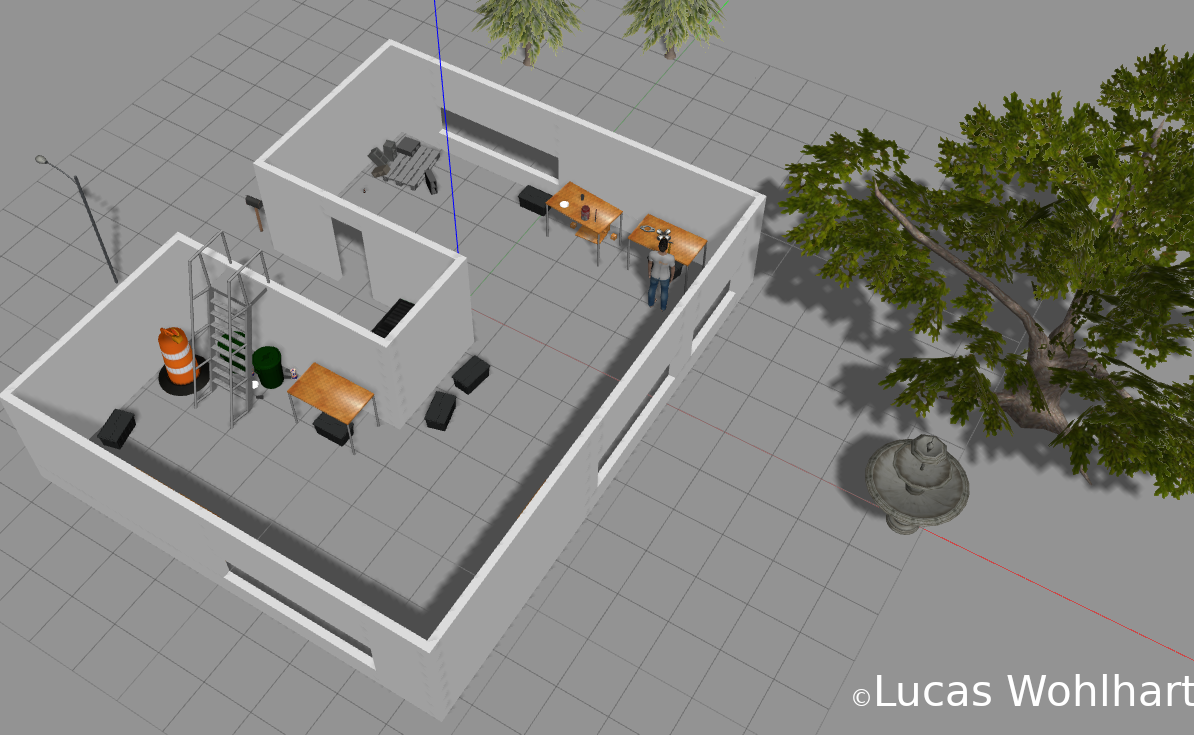
\includegraphics[width=\linewidth]{img/factory_world.png}
      \caption{Factory room world}
      \label{fig:factory_world}
\end{figure}

\subsection{Robot configuration}
The basis of the robot model is a differential drive robot modelled after the MSE6 galactic empire repair droid, taken from a previous localization project and extended with regards to its sensory capabilities. Apart from its laser range sensor mounted on top, the new model now has a front facing RGB-D camera to enable its use for RTAB-Map based SLAM. The model is shown in Fig.~\ref{fig:lw_mse6_bot_slam}.
The new frame was added to the statically broadcasted transform tree (Fig.~\ref{fig:frames}) to adjust the orientation of the camera and correclty link it to the robot model.

\begin{figure}[thpb]
      \centering
      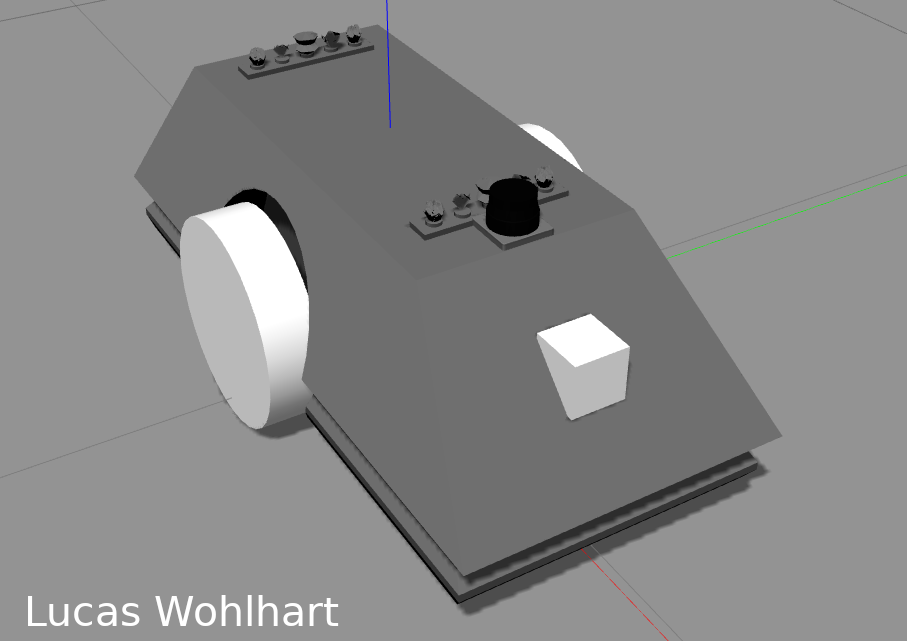
\includegraphics[width=\linewidth]{img/lw_mse6_bot_slam.png}
      \caption{LW MSE6 bot with RGB-D camera}
      \label{fig:lw_mse6_bot_slam}
\end{figure}
\begin{figure}[thpb]
      \centering
      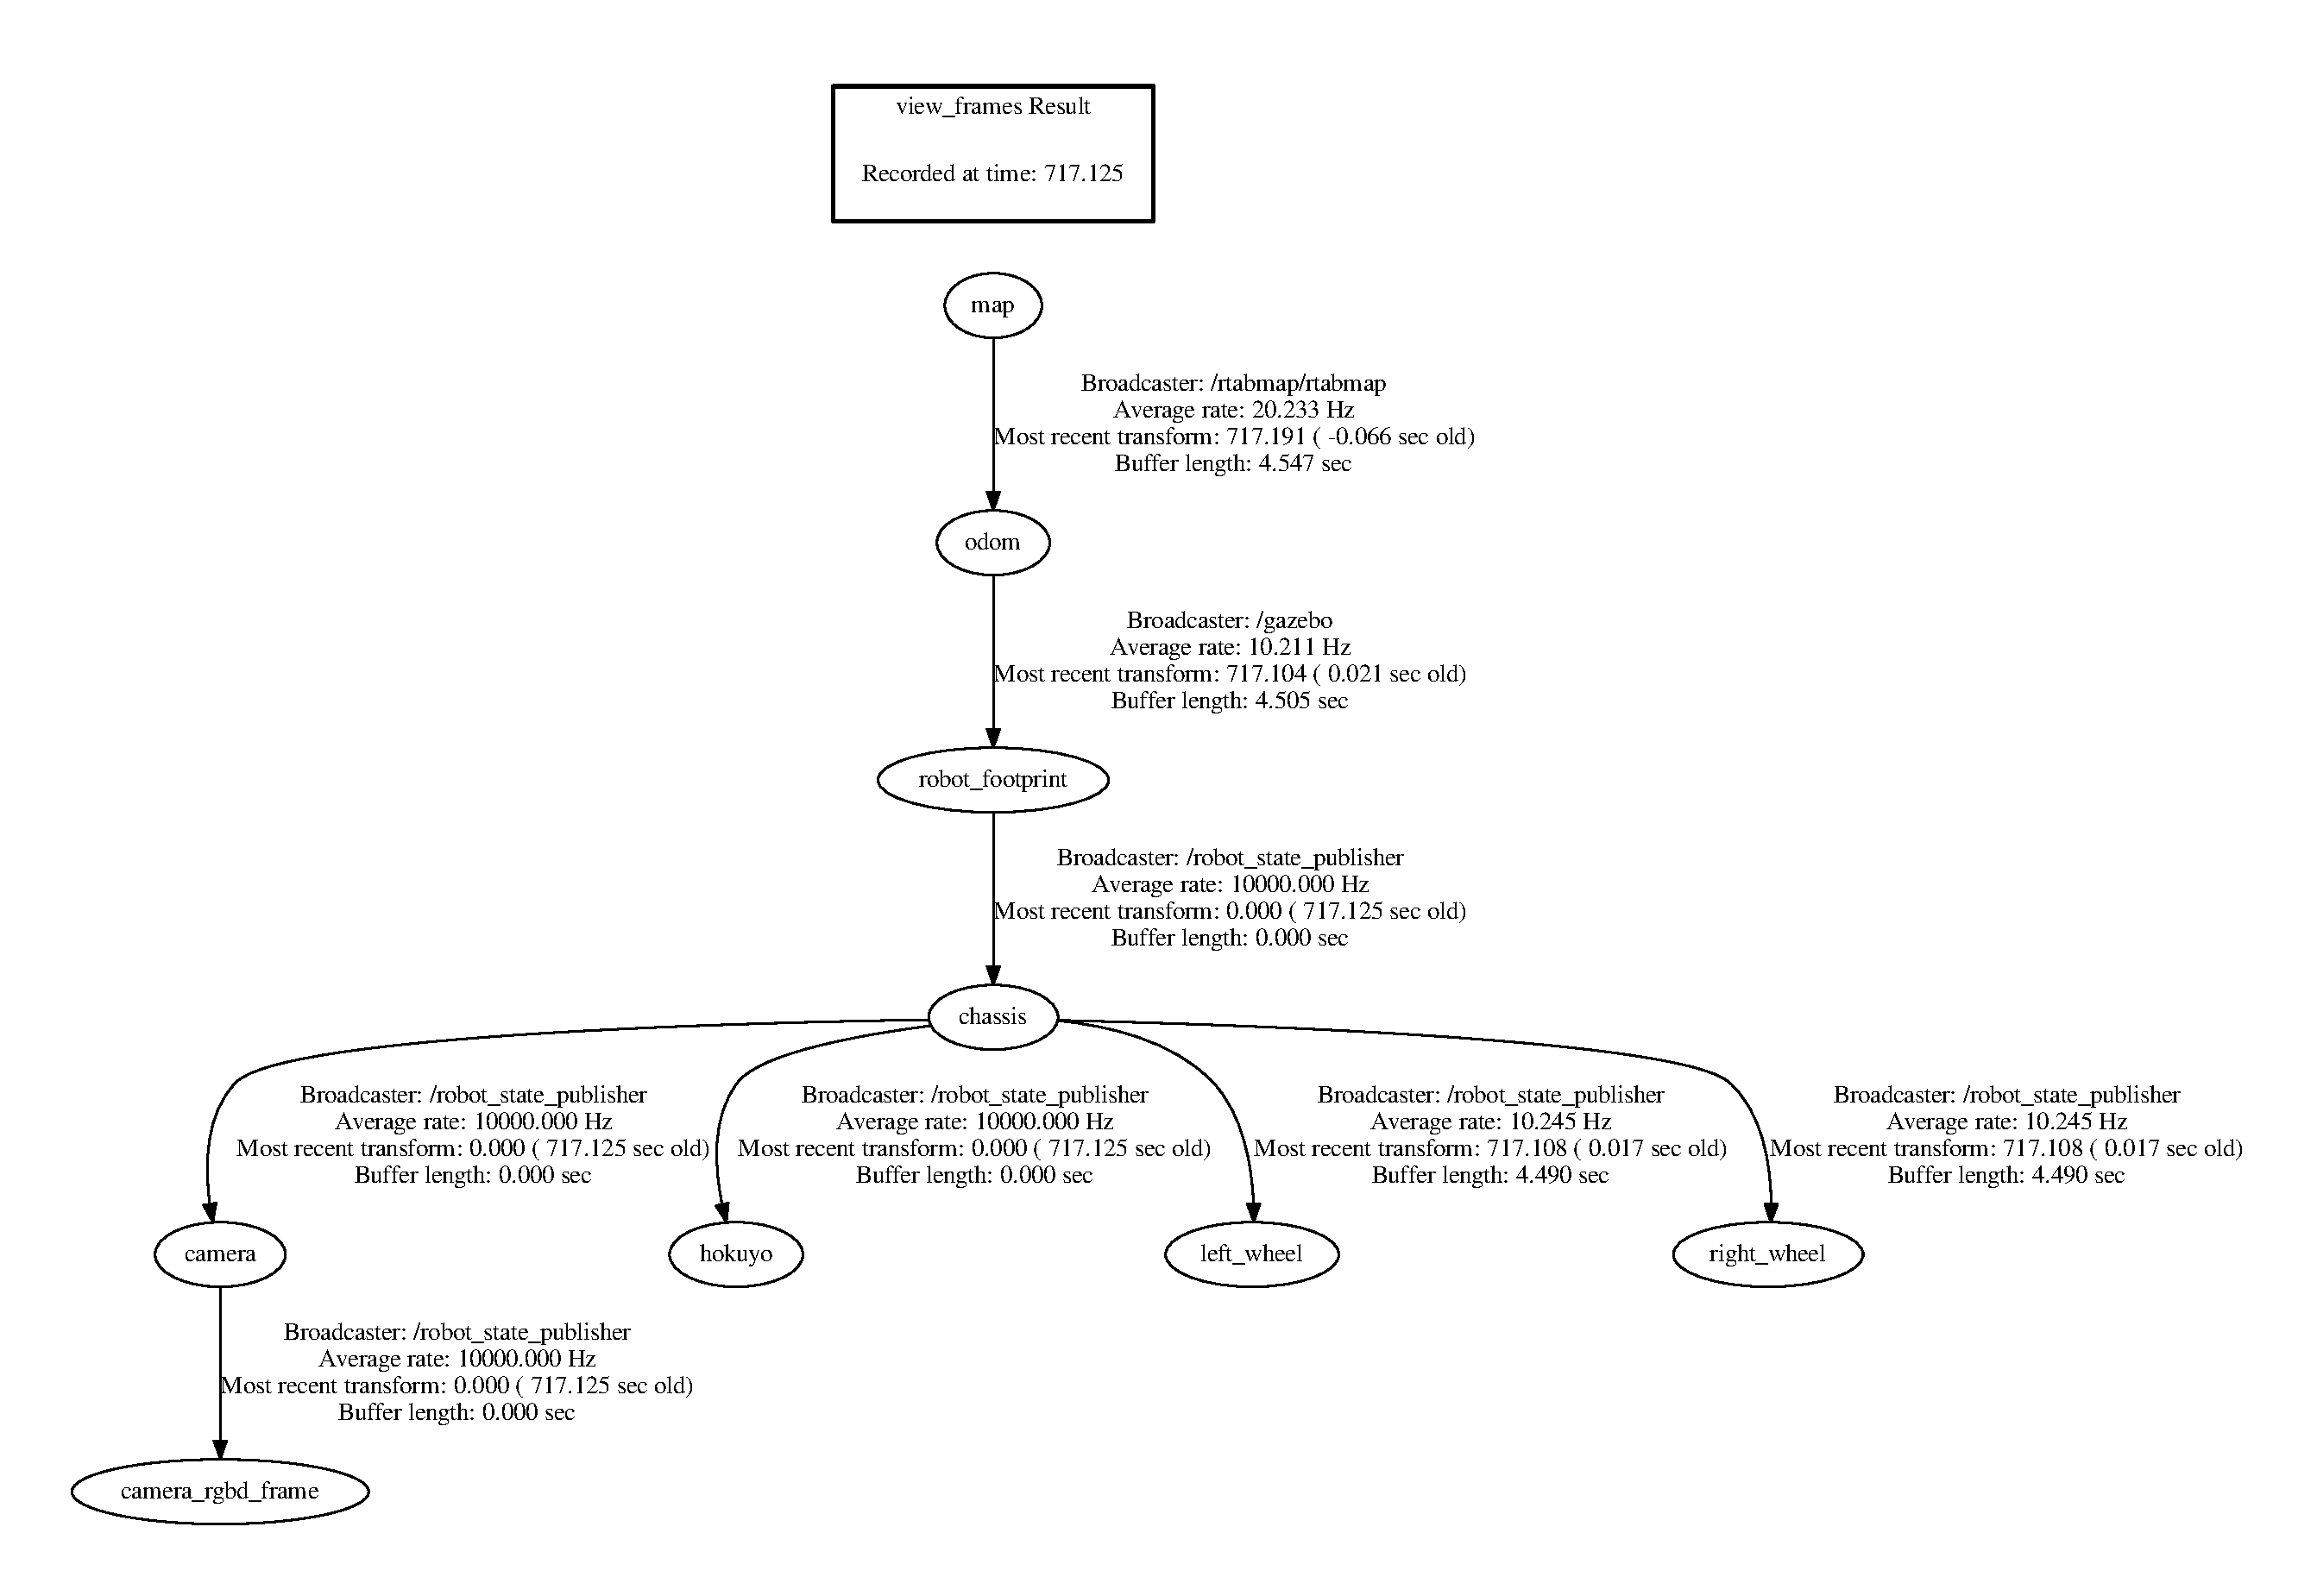
\includegraphics[width=\linewidth]{img/frames}
      \caption{Robot Frames}
      \label{fig:frames}
\end{figure}


\section{Results}

% Results - Show the results of both occupancy grid and 3D map.
% Results - The student should include the images for mapping process, final map (2D/3D) for both Gazebo worlds.

Figure~\ref{fig:kitchen_map} shows the ground truth of the provided kitchen dining world on top and the mapping result together with the estimated trajectory on the bottom.

\begin{figure}[thpb]
    \centering
    \begin{subfigure}[b]{0.45\textwidth}
        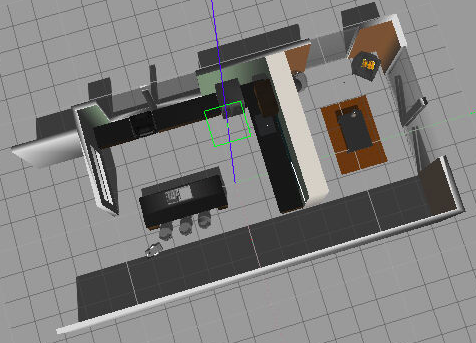
\includegraphics[width=\linewidth]{img/kitchen_map_ground_truth.png}
    \end{subfigure}
    \begin{subfigure}[b]{0.45\textwidth}
        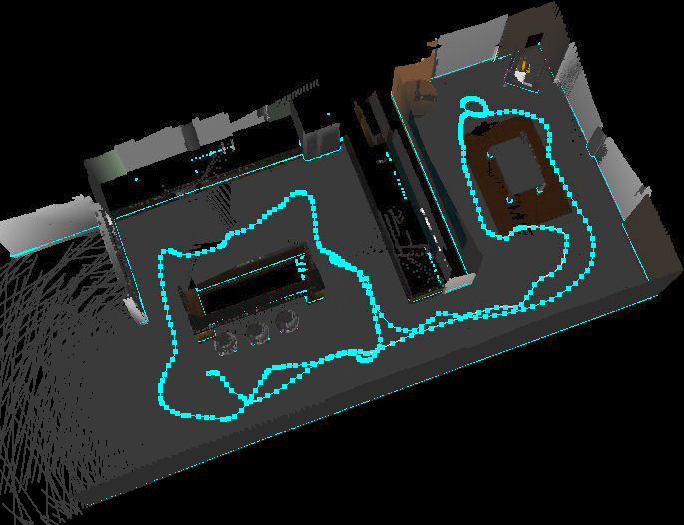
\includegraphics[width=\linewidth]{img/kitchen_map.png}
    \end{subfigure}
    \caption{\label{fig:kitchen_map}Kitchen dining world mapping: ground truth (top), mapping result (bottom)}    
\end{figure}

Figure~\ref{fig:kitchen_occupancy_grid} shows the generated occupancy grid map of the kitchen dining world as a result of the mapping algorithm.

\begin{figure}[thpb]
    \centering
    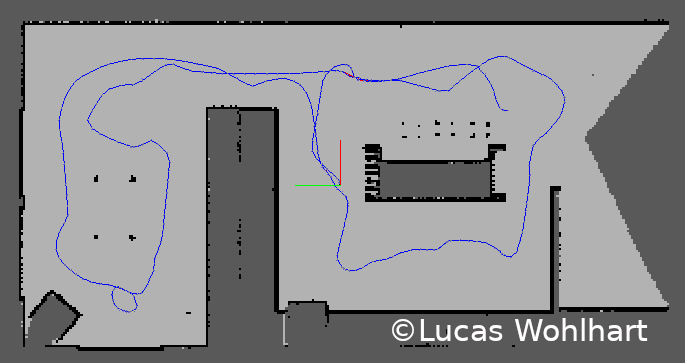
\includegraphics[width=\linewidth]{img/kitchen_occupancy_grid}
    \caption{Occupancy grid map for kitchen dining world}
    \label{fig:kitchen_occupancy_grid}
\end{figure}

Figure~\ref{fig:factory_map} shows the ground truth of the factory room world on top and the result of the mapping process as well as the estimated trajectory on the bottom.

\begin{figure}[thpb]
    \centering
    \begin{subfigure}[b]{0.45\textwidth}
        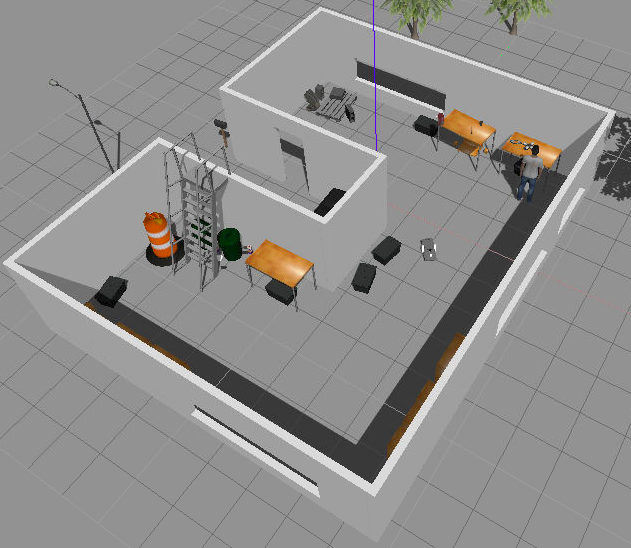
\includegraphics[width=\linewidth]{img/factory_map_ground_truth.png}
    \end{subfigure}
    
    \begin{subfigure}[b]{0.45\textwidth}
        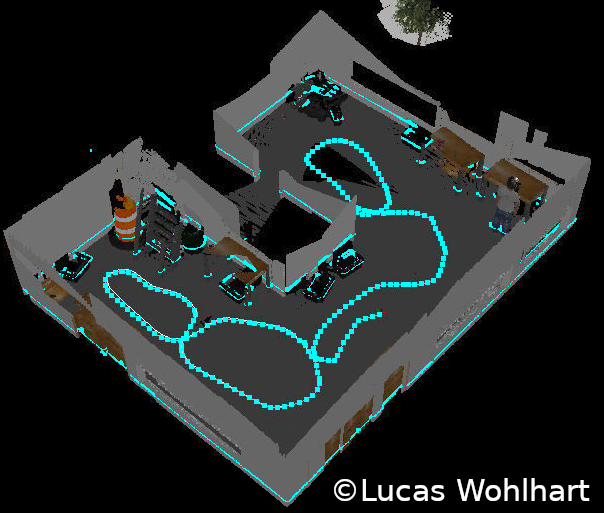
\includegraphics[width=\linewidth]{img/factory_map.png}
    \end{subfigure}
    
    \caption{\label{fig:factory_map}Factory world mapping: ground truth (top), mapping result (bottom)}    
\end{figure}


Figure~\ref{fig:factory_occupancy_grid} shows the generated occupancy grid map of the factory room as a result of the mapping algorithm.

\begin{figure}[thpb]
      \centering
      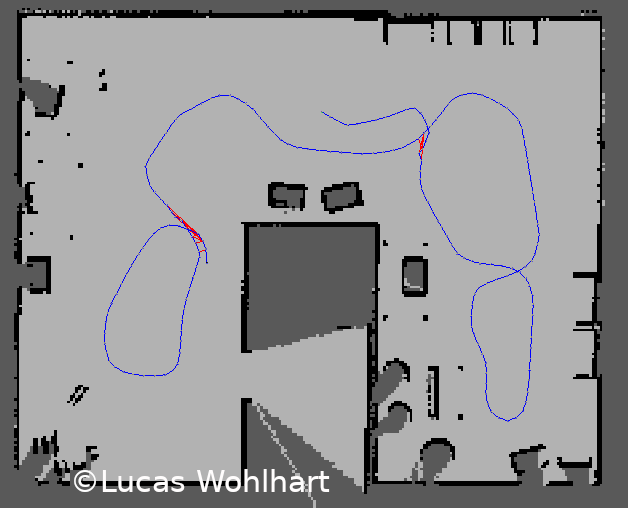
\includegraphics[width=\linewidth]{img/factory_occupancy_grid}
      \caption{Occupancy grid map for factory room world}
      \label{fig:factory_occupancy_grid}
\end{figure}

Figure~\ref{fig:factory_loop_closure} shows the successfull detection of a loop closure. One can observe the matched features in the previously encountered scene and the new observation. The RTAB-Map algorithm was able to correctly identify the features of the shelve as the previously seen shelve.

\begin{figure}[thpb]
      \centering
      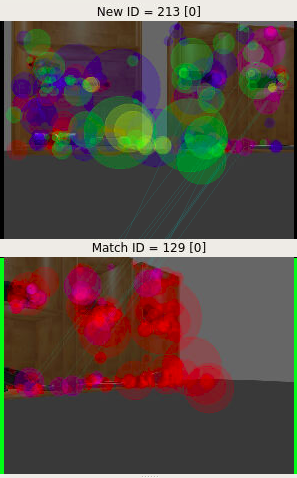
\includegraphics[width=0.65\linewidth]{img/factory_loop_closure.png}
      \caption{Detected loop closure}
      \label{fig:factory_loop_closure}
\end{figure}


Figure~\ref{fig:erroneous_loop_closure_detection} shows an erroneous detection of a loop closure due to the repetitveness of the brickwall pattern. A different corner of the world apparently also features the exact same texture causing the loop closure detection to trigger.

\begin{figure}[thpb]
      \centering
      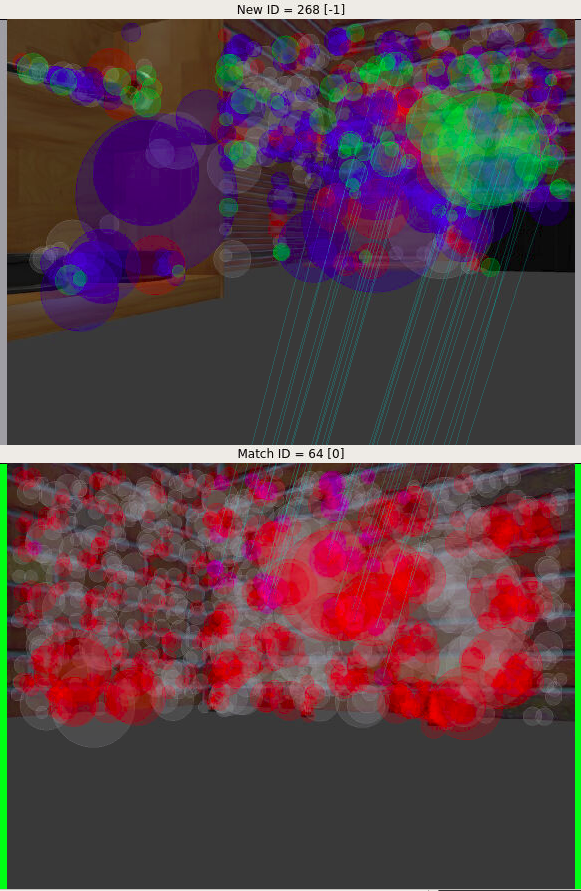
\includegraphics[width=0.65\linewidth]{img/erroneous_loop_closure_detection}
      \caption{Erroneous loop closure detection}
      \label{fig:erroneous_loop_closure_detection}
\end{figure}

Figure~\ref{fig:erroneous_loop_closure_detection_1_map} shows the resulting map after incorrectly detecting a loop closure. This false-positive can have dramatic effects on the optimization process.

\begin{figure}[thpb]
      \centering
      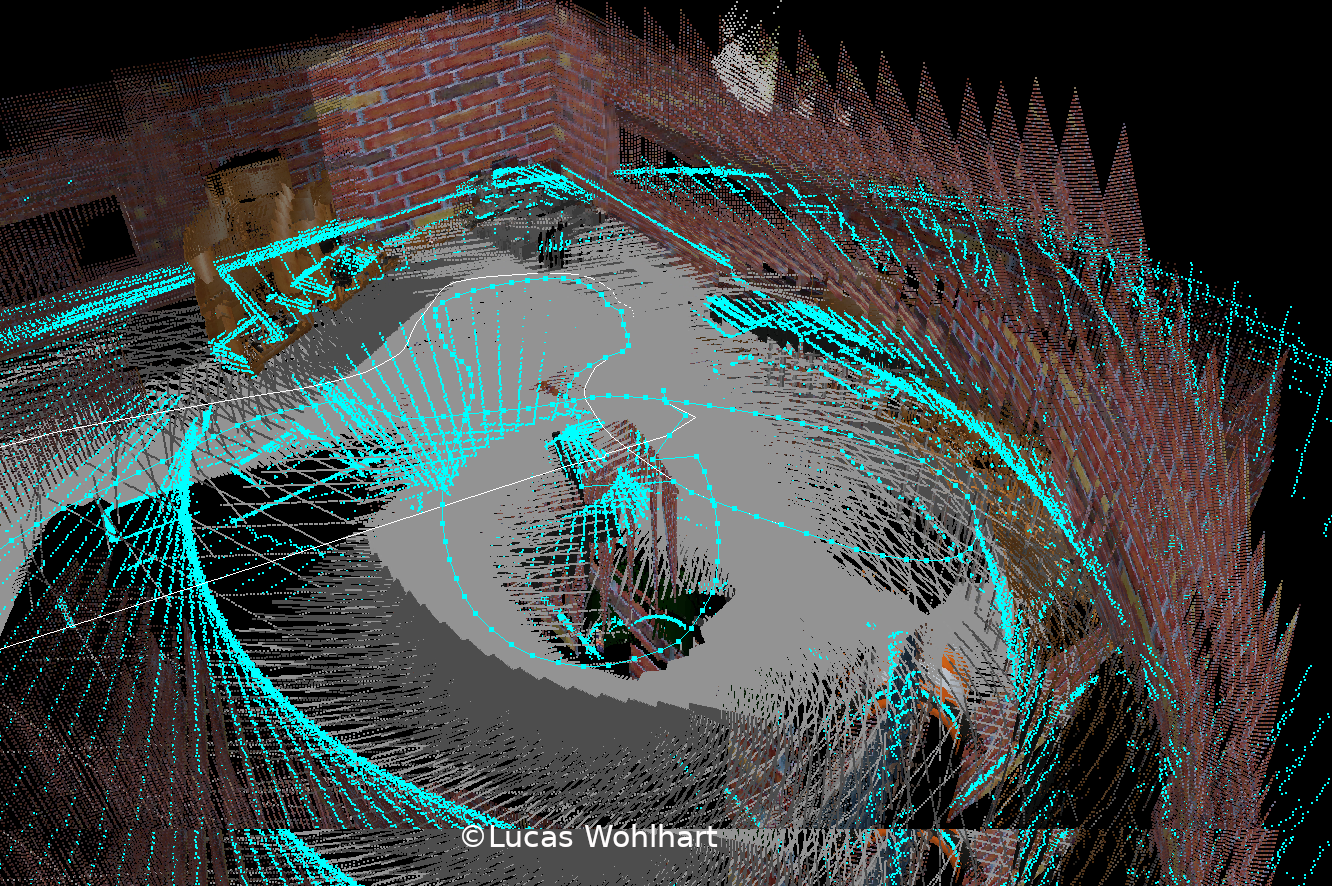
\includegraphics[width=\linewidth]{img/erroneous_loop_closure_detection_1_map.png}
      \caption{Mapping failure due to erroneous loop closure}
      \label{fig:erroneous_loop_closure_detection_1_map}
\end{figure}


\section{Discussion}

The RTAB-Map algorithm was capable of generating a very accurate map of both the provided kitchen dining world environment as well as the factory room.
The occupancy grid maps definitely provide a valuable basis for path planning and autonomous navigation in both cases and the 3D maps closely resemble their ground truth counter parts.

Loop closure detection has proven to be a valuable tool to jointly optimize parts of the graphs that belong to previously encountered locations.

However erroneous loop closure detections can also introduce problems as depicted in Figure~\ref{fig:erroneous_loop_closure_detection_1_map}. This issue is more prominent in simulated environments where textures that are reused in different parts of the wordl can have a pixel accurate resemblance. These false-positive loop detection can drastically deteriorate the mapping results.


% Discussion - What went well, what went wrong. Reflect upon the results of your robot's performance, and the performance of mapping in both worlds. Justify your answers with facts.

% Discussion - The student explains how the procedure went and methodologies to improve it. The student should compare and contrast the performance of RTAB Mapping in different worlds.

\section{Conclusion / Future work}
The RTAB-Map has proven to be a valuable to for solving the SLAM problem. 

Implementing and testing the RTAB-Map algorithm in a real world robotic application would give valuable insights in the performance of this method.

Mapping based on this method could be valuable for other type of robots such as drones or diving robots. Apart from robotics applications the approach could be an interesting tools for cartography in general.

% Future Work - Student discusses future desires with RTAB-Map. Talk about any robots and environment they applied this too.
% "Future Work - The student can discuss how they would like to leverage this tool in robotics. The student identifies other areas where mapping could be done and for what reason. Such as simulated room or physical place.
% [Optional] The student applies RTAB Mapping to a real robot."

\bibliography{bib}
\bibliographystyle{ieeetr}

\end{document}